\chapter{Discussion}
\label{discussion}

This thesis presents the argument that discourse understanding 1) shapes how people understand and interact with graphical user interfaces on the Internet; and 2) how such knowledge might be used to manipulate context, affecting comprehension and, therefore, behavior.

By analyzing GUI microinteractions in the way that we analyze linguistic discourse, it may be possible to explain some sorts of mis-understandings and even present solutions for improving user interaction design. This chapter summarizes results of experiments from the previous three chapters in context of related work in cognitive science.

While qualitative methods are extremely important for guiding a research program, it is through quantitative methods that causality is determined. While Experiments 1 and 2 focused on user comprehension, Experiment 3 concerned how knowledge about the presence of third-parties affects production. The third experiment was problematic in several respects.

\section{Summary of Findings}
\label{summaryoffindings}

 \autoref{summary-results}  summarizes results for all experiments in this dissertation.


%% LyX 2.0.6 created this file.  For more info, see http://www.lyx.org/.
%% Do not edit unless you really know what you are doing.
%\documentclass[english]{article}
%\usepackage[T1]{fontenc}
%\usepackage[latin9]{inputenc}

%\makeatletter

%%%%%%%%%%%%%%%%%%%%%%%%%%%%%% LyX specific LaTeX commands.
%% Because html converters don't know tabularnewline
%\providecommand{\tabularnewline}{\\}

%\makeatother

%\usepackage{babel}
%\begin{document}
%B%
%\begin{table}
%\begin{center}
\begin{longtable}{l p{10cm}}
\caption{Experiment Design} \\
1A & 2x2x2 between group posttest-only design where the control group is
presented with a set of textual expressions and asked to answer
questions about their meaning. Treatment groups are presented with either textual expressions or a dialog box expressing the same set of choices and asked the same
questions. Independent Variables: Modality, Deontic force, Attitude
toward privacy. Dependent Variable: Pragmatic implicature\tabularnewline
\hline 
1B & Between group posttest-only design where two groups are presented
with a cookie banner and later asked about whether or not they believe
the website placed \textquotedbl{}cookies\textquotedbl{} in their
browser. The treatment group is presented with feedback about the
consequence of their action / non-action following presentation of
the banner. Independent Variable: Feedback. Dependent Variable: Pragmatic
implicature.\tabularnewline
\hline 
2A & Between group posttest-only design where five groups are presented
an advertisement in the context of a webpage and asked to identify
hyperlinks. Treatment groups are presented an advertisement with embedded
image icons at four levels (known icon + different company, unknown icon, known call-to-action (CTA), ``DAA opt-out icon'') while the control group is presented with an embedded image from the same company as the advertiser. Independent
Variable: Icon type. Dependent Variable: Indexicality of icon. \tabularnewline
\hline 
2B & Between groups posttest-only design where three groups are presented
an advertisement in the context of a webpage and asked to identify
hyperlinks. Treatment groups are presented an advertisement at two
levels (iconic CTA, textual CTA) while the control group is presented
with an advertisement with no CTA. Independent Variable: Modality
of CTA. Dependent Variable: Click target.\tabularnewline
\hline 
3 & Between group repeated measures posttest-only design where a control
group is asked to respond to a survey containing questions relating
to activities (using questions drawn from \cite*{Acquisti:2012tp}; embarrassing, socially / ethically questionable, illegal). Participants
are notified in a privacy statement that there may be ad trackers
on the site. The treatment group receives exactly the same notification
and survey. However, tracker presence is indicated in a visual display
throughout the participant's session. Independent Variable: Visual
presence. Dependent Variable: Propensity to respond in the affirmative
to engaging in specific behaviors.\tabularnewline
\hline 
\end{longtable}
%\end{center}
%\end{table}
%\end{document}



\section{Discussion of Results}
\label{discussionofresults}

Pragmatic theory distinguishes between several types of factors affecting comprehension and reasoning:

\begin{enumerate}
\item \emph{Social dimensions} of discourse (e.g., cooperative principle; intent; norms; participant roles)

\item \emph{Knowledge} (e.g., subject \slash  content matter; deictic relations)

\item \emph{Saliency} (e.g., cognitive saliency of referents; task saliency)

\end{enumerate}

Attitudes and beliefs also affect reasoning as described by  \citet{Kahneman:1984td},  though these do not fall under the purview of pragmatic theory.

Experiment 1 concerned pragmatic reasoning where subjects reasoned over both textual and mixed-modal content. Not only were mixed-modal representations subject to the same sorts of pragmatic inferences as purely textual representations, small changes in language and content were shown to have significant effect in understanding and, ultimately, behavior. Furthermore, immediate feedback was seen to affect comprehension. 

Experiment 2 primarily considered the role of knowledge (icon referent) in the inference of an indexical relation. By manipulating an icon embedded in a graphical ad, I looked at whether knowledge about that icon (against a background context) played a role in its interpretation. In the pilot, it seemed this was the case, but in the actual experiment, any effect was too small to see. The primary difference was that in Experiments 2A and 2B, the ad image was embedded in the larger context of a news article while in the pre-pilot, the ad was considered in isolation.

Finally, Experiment 3 concerned whether manipulation of visual presence (and, therefore, participant role) would affect responses in a task measuring propensity to disclose sensitive information. In theory, this should be the case. However, I believe elements of task context (including use of AMT) and user knowledge may have affected results.

Below I discuss each experiment in more detail.

\subsection{Experiment 1: Modal Dialog Boxes}
\label{experiment1:modaldialogboxes}

Assuming a common set of principles driving understanding of both multimodal and textual content, people should be as sensitive to implicature in multimodal messages as linguistic messages. In fact, it appears not only is this so, but to a higher degree. This has clear implication for design: \emph{user choices made using non-forced choice modal dialog boxes may be mis-understood}.

Why might people mis-understand the meaning and consequence of choice?

 \citet{Evans:2003gp}  asserts evidence for two types of thought processes: \emph{heuristic} and \emph{analytic} (also referred to as System 1 and System 2, as well as, Type 1 and Type 2 in  \citealp{Kahneman:2011tc,Manktelow:2012tx}, respectively).  Much of this work is based on studies of deductive reasoning. For example, the Wason selection task  (\autoref{wason}; \citealp{Wason:1960wt})  asked people to select cards which falsify the statement in (a). Subjects were shown 4 cards and told that each card had a letter on one side and a number on the other. The correct answer is A and 7, though only 10--20\% of people answered correctly  \citep{Wason:1960wt}.  However, when given task (b) and told they play the role of a police officer checking people drinking in a bar, about 75\% were successful  \citep{griggs1982elusive}.  

These studies and others, point to a belief bias where belief is seen to affect reasoning about logical arguments. Similarly, a matching bias is seen in more abstract tasks; a matching bias is one in which one tends to select answers which contain lexical content which matches content over which one is reasoning (e.g., selection of A and 3 as answers in the Wason task mentioned earlier). Such biases provide support for a heuristic, autonomous system for reasoning which takes into account knowledge and belief. Other processes relating to the social dimensions of language use, also appear to be automatic (discussed in the next section).

There are several theories of reasoning that aim to explain this sort of phenomenon:  \citet{Cheng:1985ww}  propose domain specific knowledge structures (pragmatic reasoning schemes) which are remembered and applied from previous experience to new situations;  \citep{JohnsonLaird:1983vt}  argues that people create mental models of assertions and rely on these to reason; and,  \citep{Cosmides:1989dq}  proposes a ``social contract'' algorithm which is specialized to assess costs and benefits in social exchange.


\begin{figure}
\centerline{
  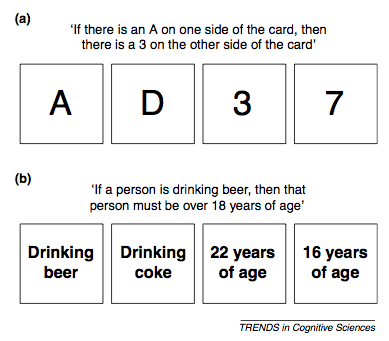
\includegraphics[scale=.75]{chapter8.tex/wason}
  }
\caption{Wason Selection Task (Image credit: \citealp{Evans:2003gp})}
\label{wason}
\end{figure}


Whether through discourse models, pragmatic reasoning schemas (PRS), or other heuristics, people are adept at reasoning over discourse with little apparent effort or thought. In all conditions, subjects were subject to implicature (see  \autoref{exp1-raw}  for raw results). What is surprising is how sensitive implicature is to small changes context. Across eight conditions, interpretation of implicature varied from 38\% (text, pictures, on\slash off) to 84\% (graphics, cookies, on\slash off). 

Experiment 1B was concerned with how people interpret the question presented in Experiment 1A --- but in the context of decision-making. In Experiment 1A, subjects were asked what they thought `cancel' or `x' meant. They had time to reflect and reason. 

In Experiment 1B, subjects were asked to think about what they thought their choice meant immediately after making a decision. Surprisingly, a great number of subjects attended to the dialog box and chose to respond (30--35\%). This is likely a higher percentage than what might be expected of the population of users on the Internet as a whole. Only 22\% of those in the control condition made an inference about the presence of cookies based on their choice. Of those that didn't, 45\% of those that thought there were cookies answered ``there are probably always cookies'' and 72\% of those who didn't think there were cookies said they used an ad blocker. The large number of turkers who believed there were always cookies suggests a belief bias. And the number that used ad blockers strengthens this: turkers are very knowledgeable of privacy issues.

Of those that did interpret an implicature, it's possible a matching bias was in effect. It is also possible subjects short-cut reasoning using a simple schema or model. Either way, subjects may have reasoned:

\begin{itemize}
\item "I didn't select NO and I didn't select YES, therefore neither NO nor YES." 
\item Or, perhaps, "I didn't select NO, therefore YES." 
\item Or, similarly, "I didn't select YES, therefore NO."
\end{itemize}

Why one would select one or the other of the latter two is a good question. Either way, they made a choice without understanding the consequence.

The number of people making an inference about the presence or absence of cookies based on choice was lower than expected. The high ``participation'' for choice seems likely due to the nature of the task environment: workers may be likely to cooperate and take action on prompts because they have agreed to do work for pay. 

Regardless, there were far fewer inferences made when feedback was provided. \emph{Without immediate feedback, odds were 6.6 times higher that subjects understood an implicature to be true}.

\subsection{Experiment 2: Embedded Icons in Graphical Ads}
\label{experiment2:embeddediconsingraphicalads}

Experiment 2 was also about pragmatic reasoning, though not the sort associated with logical or semantic reasoning. In the pre-pilot to Experiment 2, participants examined advertisements and were asked to click wherever they thought there might be a hyperlink. Hyperlinks associate an object on a page or in a scene with other content. When there are no visual cues, such a relation largely derives from knowledge people have about the meaning of an object and to what it might refer. Even so, judgements seems to be context sensitive.

In Experiments 2A and 2B, participants were given a task in context --- advertisements were embedded in a news page. From Experiment 2A, it seems that an icon embedded in a graphical advertisement is not likely to be considered indexical, regardless of what that icon represents --- except in the case of the FaceBook icon which is an explicit ``call-to-action'' (like \slash  share) associated with all sorts of different content on the Internet. I had hypothesized that several factors might be at play: 1) icon salience by a contrastive relation (visually \slash  semantically) with the background ad; 2) knowledge that the icon is indexical to some brand; and, 3) recognition of a signal or ``call to action'' for clicking. In 2A, the only icon which was considered indexical was the FaceBook icon, exhibiting all three properties. It is possible that estimating for a medium effect size for an ad in context, was not enough to see whether (1) and (2) made a difference, independently.

Experiment 2B attempted to determine whether explicit indexicality affected behavior. Would an ad with a CTA that had the form of a button invite a user to click directly on the button? In the pre-pilot, this appeared to be the case, but there was no effect in the embedded context of Experiment 2B. Again, it is possible that the embedding context (ad within a news page) had an effect, potentially reducing the effect size. It is also possible that we may see no effect with more savvy Internet users but would see one with those who are less savvy.

Regardless, these insights were useful in understanding why the AdChoices icon may not be effective for conveying intent to users. Size has less of an effect than one would imagine. More important, \emph{embedded graphics in ads may not be considered indexical by default}. At least not today. As users become accustomed to certain associations and patterns, they may well adapt.

\subsection{Experiment 3: Third-Party Bystanders Versus Eavesdroppers}
\label{experiment3:third-partybystandersversuseavesdroppers}

Experiment 3 attempted to address whether participants might change their behavior depending on whether they thought advertisers were actively observing them (i.e., the difference between non-ratified bystanders versus non-ratified, eavesdroppers). If the treatment group behaved differently, this would lend support to the notion that participants aware of being monitored, changed their behavior in response. However, it appears that both groups were equally cognizant of the potential for third-party monitoring. 

Two years ago, turkers, along with most people on the Internet, had little knowledge of OBA. In a recent survey conducted by  \citet{Lease:2013vq},  at least some AMT workers were aware of the potential for leakage of personal identity via workerId: worker identity is not completely private and can be found in web searches. The survey in this dissertation revealed that more than 90\% of turkers knew what cookies were, and what's more, nearly 75\% used ad blockers. Though most of them felt ``more private'' on the Internet at home than when sitting in a public setting, they seem to have a heightened sensitivity toward privacy issues which may have affected the outcome of this experiment.

Video gaming site owner, Niero Gonzalez was surprised to find that nearly have of his 3 million visiter a month blocked ads  \citep{Hill:2013wp}.  From the same source, PageFair says that ad blocking is growing at a rate of 43\% per year. Given how knowledgeable my sample was about Internet privacy and tracking technology, few would consider their communications anonymous. Moreover, given the contractual relation between the requester and worker on AMT, only those willing to share sensitive information would be willing to accept such a HIT. Quite possibly, this rendered the question of bystanders versus eavesdroppers irrelevant.

 \citet{Ur:2012ws}  deliberately recruited non-technical people who were little aware of tracking on the Internet. By contrast, turkers are very aware of tracking. Perhaps, results would have been different two years ago. In Experiment 3, the sample studied was likely not representative of the larger population of Internet users. From this perspective, AMT was not a suitable recruitment platform. However, turkers may reflect what we will see from the majority of users in time. And, good or bad, what feels creepy now, may not after longer familiarity.

\subsection{Use of AMT}
\label{useofamt}

Only recently have researchers in pragmatics and sociolinguistics adopted controlled experimentation (and on platforms such as Mechanical Turk) for the study of discourse phenomena.  \citet{Assessingthepragma:2011ug}  note that pragmatic phenomena are difficult to study because of the many contextual parameters that affect understanding. Crowdsourcing platforms such as AMT now make it possible to vary context parametrically without excessive expense and time. In a study of scalar implicature,  \citet{Assessingthepragma:2011ug}  found that simply changing the task instructions to ``quality control'' altered the proportion of responses in an implicature-oriented situation. Though such methods look useful for testing UI design comprehension, there is much to learn about how to best do this.

\subsection{Potential Population Bias}
\label{potentialpopulationbias}

In both methods and presentation of experiment results, I've noted attributes or characteristics of the AMT population that makes it difficult to typify them as characteristic, non-privacy aware Internet users. Other potential issues, regarding use in cognitive and other experiments were also noted. Like other researchers, I performed tests varying payment looking for quality differences across collection events. However, differences between results in Experiment 2 pre-pilot and Experiments 1 \& 2 suggest that there may be another factor.

 \citet{Rush:1978tw}  noted that subjects that volunteer for pay tend to commit more errors of omission on selective attention tasks. They suggested that paid subjects might working more for task completion than success. In experiment 2B, I offered a 3-minute task for 15 cents. Even when I added collection events increasing payment to 25 cents, and shortening the task by omitting demographic questions, I saw no difference in results. Yet, corresponding samples from the pre-pilot at 75 cents (15--20 minute task) obtained different results. It also possible some other variable might be in play. Perhaps, some workers (e.g., those focused on pay) simply prefer more attractive tasks (easiest; highest reward to time ratio). These tasks are consumed quickly leaving ``less attractive'' tasks for other turkers to tackle. This question remains future work.

\section{Cognitive Architecture}
\label{cognitivearchitecture}

As central goal of this dissertation is to provide support for the notion that user interaction with graphical user interfaces involves discourse processes, a basic discussion of the cognitive architecture facilitating language understanding is essential.

\subsection{Situation Models}
\label{situationmodels}

Language, perception, and action are closely aligned  \citep{Lakoff:2008tq}.  In recent years there has been much support from brain imaging. For example,

\begin{itemize}
\item Activity in pre-motor cortex suggests a causal link for the understanding of action verbs \citep{Willems:2011gp};
\item High manipulability words evoke greater activation in the motor cortex \citep{Madan:2012ja};
\item Perspective in pictures has an effect of learning \citep{deNooijer:2013jc};
\item Evidence of the activation of modality specific representations during discourse show that mental imagery occurs during discourse comprehension.\citep{Kurby:2013tp}
\end{itemize}

Furthermore, theories of language comprehension suggest that text comprehension involves the constructions of a mental representation of events described in text  \citep{Zwaan:2002va,Kintsch:1978vz,vanDijk:1990tc}.  

In semantics, a propositional representation conveys logical meaning using lexical and grammatical features. Depictive representations, on the other hand, do not encode such relations symbolically. Propositional and depictive representations make different sorts of information explicit and accessible  \citep{Kosslyn:2006tj}. 

 \citet{Kosslyn:2006tj}  make the argument that visual imagery evokes many of the same processing mechanisms in visual perception. While sensory visual perception is driven by sensory input, visual perception makes use of stored information.

Mental representations form the building block of situation (viz. discourse) models  \citep{Zwaan:2002va,Zwaan:2013wk}. \citet{Zwaan:2013wk}  is careful to distinguish these from the notion of schemas such as learned stereotypical ``scripts'' (e.g., greeting rituals) in interaction. Individual elements of a script have mental representations, and schemata themselves may be used in the construction of models.

Discourse models are necessary for explaining language processing. Discourse understanding requires readers to integrate and recall information across spans of sentences. Moreover, discourse models account for how representations are constructed across modalities.  \citet*{Gernsbacher:2013vl,Zwaan:1999td}  found a correlation in comprehension across three modalities (written, auditory, and visual) suggesting that mental representations are independent of modality and used in the integration of verbal and visual information. 

\subsection{Interactive Alignment and Priming}
\label{interactivealignmentandpriming}

In a theory of \emph{interactive alignment},  \citet{Pickering:2003uy}  attempt to account for dialogue as the more basic framework for language comprehension and production over monologue. They argued that linguistic representations become aligned at many levels, as a result of an automatic processes. This is accomplished by ``dialogue routines'' which simplify language production and comprehension by short-circuiting decision-making processes.

Essential to successful dialogue, is alignment of situation models. Doing so, eliminates the need for speakers to actively maintain a listener model. \citet{Pickering:2003uy} give evidence of this as alignment in coordinating referring expressions in dialogue through a model of common ground \citep{Brennan:1996ud,Clark:2003uw,WilkesGibbs:1992ui}. They also give examples of alignment across other levels of abstraction: articulation \citep{Bard:2000bp}, syntax \citep{Branigan:2007ug}, and comprehension. 

Though the goal of monologue (spoken or written) is not aligned representations, readers draw inferences on the basis of knowledge of the writer --- and the writer must infer what the listener has inferred. Only through interaction, do processes of feedback help interlocutors recognize and correct mis-understanding  \citep{Clark:1996tm}.  

Citing  \citet{Levelt:1993tk} and \citet{Dell:1986vk}, \citet{Pickering:2003uy}  point out that it is not only advantageous to avoid levels of representation in comprehension but also in production. Noting the very repetitive nature of dialogue, they discuss the implication of ``routines'' in alignment processes. Through shared routines (repetitive expressions, lexical items, etc.) language production is eased by the prior activation of relevant lexical and syntactic representations. A prediction of their account is that word frequency effects are reduced by accessibility in dialogue contexts. That is, less frequent meaning becomes more accessible than more frequent meaning in the local context of dialogue. Such affects are facilitated through priming  \citep{Bargh:2006bo}.  ``Language perceivers implicitly learn the statistical regularities in their linguistic input, and they use this prior experience to guide comprehension of subsequent language''  \citep{MacDonald:2013bx}. 

This is relevant not only to the acquisition of lexical expressions, but also the acquisition of graphical symbols. ``Through the grounding process, interactive graphical communication enables participants to develop symbolic representations from what started out as primarily iconic representations''  \citep[p. 4]{Garrod:2007wk}.  Experiments 1 and 2 of this dissertation concern mental representations derived from both linguistic and graphical elements. Moreoever, composite components such as modal dialog boxes and graphical advertisements have become routinized by ``fluent'' Internet users. As  \citep{Bargh:2006bo}  notes,

\begin{quote}
... the study of language comprehension and production has provided social cognition with highly useful models that have enabled us, over the years, to discover 'new' and important social psychological phenomena. Given this stellar track record it might be the case that the underlying mechanisms of language production and of social behavior production are one and the same. \citep[p. 16]{Bargh:2006bo}
\end{quote}

And, particularly relevant to new work presented here:
\begin{quote}
"One might speculate that language pragmatics on the one hand and goal directed activity in social contexts on the other are derived from a common set of rules whose aim is to enable members of complex social organizations to interact." \citep[p. 105]{Girotto:1990va}
\end{quote}


\section{Themes for Future Areas of Study}
\label{themesforfutureareasofstudy}

Each of the experiments described here present opportunities for future, interesting follow-up studies. However, I will present them in the context of several broad themes.

\subsection{Micro-Interactional Design Patterns}
\label{micro-interactionaldesignpatterns}

Interacting with graphical user interfaces (GUIs) sometimes feels conversational and sometimes not. A dialogue box that asks a yes-no question doesn't seem that much different from a verbal yes-no question. But file selection prompts don't feel as natural.

When we speak in our own language about everyday matters, we speak effortlessly with little thought about how to produce an utterance and little thought about how to understand one. It's a bit different with written language. We endure years at school learning to read and write properly, following style guides which we memorize and practice endlessly until we know how to recognize and avoid passive constructions --- as well as generate them with practiced ease. Reading and writing text is just not as intuitive as speaking conversationally and most people require years of practice to achieve any competency.

When GUIs sprang into public awareness in the 70s and 80s, it became possible for people to interact with a computer without having to learn seemingly arbitrary complex commands typed into a terminal window. GUIs made sense. You could point and push buttons. An icon was a symbol that stood for something meaningful like a ``program''. And there was plain old English language mixed in with icons and graphics (since GUIs originated in the United States). GUIs felt natural.

During all of the hype of GUI-based interfaces, software developers learned to adopt the notion of software patterns. The idea was to document shared knowledge of best practices for solving common or typical problems in software design. A software pattern is a fantastic concept for anyone learning to write software. Writing software and designing UIs has much in common with learning how to read and write text. It requires a lot of practice before you become any good at it. Software design patterns help new programmers speed up the process so they don't have to figure out how to solve every problem encountered through trial-and-error.

When desktop computers became really popular --- and web interaction more so in the 2000s, some software engineers began to specialize in ``front-end'' development. Anyone learning web interaction might consult the Yahoo UI design pattern library while developing a new web application. In fact, Yahoo's purpose for its design pattern library was to solve a business problem. They wanted a way to communicate standards across development teams in order to increase ``consistency, predictably, and usability'' across their site --- and their brand  \citep{Leacock:2005ut}. 

Human Computer Interface (HCI) guidelines and design patterns are intended to capture specific problems, examples, usage, rationales, supporting research, standards, etc. Patterns range across stylistic conventions (e.g., page headers and footers), attentional mechanisms such as animation, navigation and organization, layout, common functions such as registration or login, and even more complex patterns such as social sharing and feedback. 

In addition to useful, everyday patterns, the notion of \emph{anti-patterns} and  \textit{dark patterns}\footnote{\url{http://darkpatterns.org}}  document practice in common use which may be ineffective (anti-patterns) or ethically questionable (dark patterns) patterns.

When we learn language, some concepts and patterns become \textbf{entrenched} with frequent use. So, for example, the phrase ``I don't know'' is not something most of us have to think about before uttering. The grammatical construction I (subject) + do (1st person aux verb) + negation + know (infinitive) is not something you have to think about assembling before you say it. Such forms become \textbf{routinized} through repeated activation and use --- such that both \emph{production} and \emph{understanding} require less cognitive effort and is more automated  \citep{Pickering:2003uy}. 

This sort of automatization is not limited to conversational speech. Routinization happens at many levels of production and understanding. For example, when you see a familiar word like ``key'', pronunciation is automatic. It also interacts with syntactic chunks such that when someone says, ``cat in the  \underline{   }",  you anticipate ''hat``  \citep{Pickering:2003uy}. \\

\begin{figure}
\centerline{

\includegraphics[scale=.5]{chapter8.tex/cathat}
}
\caption{Cat in the Hat}
\label{cathat}
\end{figure}

When you see a tall hat with red and white stripes as in  \autoref{cathat},  you may immediately think cat-in-the-hat, as well as ''cat``, ''Dr. Seuss", and any number of related concepts. According to  \citep{Pickering:2003uy},  \textbf{priming} may occur at different levels including lexical, syntactic, semantic, and situation. 

Routinization isn't limited to long-term memory. Suppose you are having a conversation with a friend. You are talking about a movie of which neither of you can remember the name. So you say, ``that movie with Harrison Ford''. It would not be surprising if your friend then referred to the same movie as, ``the Harrison Ford movie''. You can routinize a reference to something during the course of an interaction in order to communicate more easily.

Priming is also applicable to GUI patterns. When the GUI presents a dialog box like the one below, it is familiar. It offers a choice (1) or (2). Typically, the choice is binary --- cancel or accept; yes or no; permit or deny, etc. You read the text and make a choice. 


\begin{figure}
\centerline{
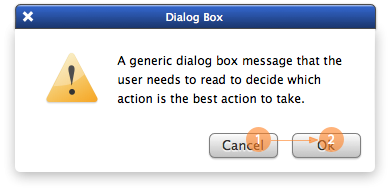
\includegraphics[scale=.5]{chapter8.tex/dialog1}
}
\caption{Image credit: \url{http://uxmovement.com/buttons/why-ok-buttons-in-dialog-boxes-work-best-on-the-right/}}
\label{dialog1}
\end{figure}


Once you've seen  \autoref{dialog1},  you don't have to ponder over similar dialog boxes each time you encounter one. In fact, the more often you see and recognize a design pattern, the more entrenched it becomes. 

What is the difference between an interaction design pattern and linguistic pattern? Well one obvious difference is while we use language all day long, only a few of us know how to produce UIs. And when people interact with UIs, they aren't interacting directly with the designer. So the designer doesn't get direct (or continuous) feedback on how well the user understands the interaction. Production is not directly linked to comprehension in a realtime feedback loop like face-to-face dialog; it is a bit more like interacting with monologue text. This means that patterns are not aligned and refined in the same way. 

Interaction design patterns help improve communication, but because they are easily modified by the designer with no direct feedback about how such changes affect a user's comprehension --- there is the possibility for non-obvious error. 

In fact, there might be a lot of information packed into a dialog box. Dialog boxes don't have to be simple binary choices. The UI designer can make a dialog box for any purpose.  \autoref{dialog2}  illustrates a very simple one where explicit choice is omitted. 


\begin{figure}
\centerline{
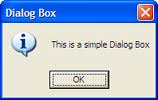
\includegraphics[scale=.5]{chapter8.tex/dialog2}
}
\caption{One Choice and Ignore?}
\label{dialog2}
\end{figure}


 \autoref{dialog3}  illustrates an example of where the designer decided that a form could be a dialog box. What happens if I don't fill something out right?


\begin{figure}
\centerline{
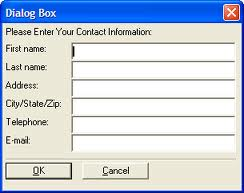
\includegraphics[scale=.5]{chapter8.tex/dialog3}
}
\caption{Dialog Box or Form?}
\label{dialog3}
\end{figure}


 \autoref{dialog4}  is the familiar open document dialog. Sometimes you can open more than one document but there is no way to know without trying it.


\begin{figure}
\centerline{
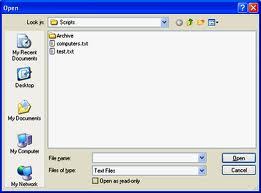
\includegraphics[scale=.5]{chapter8.tex/dialog4}
}
\caption{Select File Dialog}
\label{dialog4}
\end{figure}


 \autoref{dialog5}  is complex dialog that combines the basic cancel, accept pattern with other buttons and choices. From experience, I expect that I can do a bunch of things and then choose ``OK'' or ``Cancel'' when I'm done. But it requires a bit more thought on my part --- and also a bit of trust where if I spend a lot of time on this and then mess something up, I don't know what will happen.


\begin{figure}
\centerline{
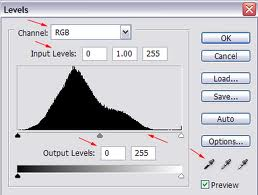
\includegraphics[scale=.5]{chapter8.tex/dialog5}
}
\caption{Complex Dialog Box}
\label{dialog5}
\end{figure}


 \autoref{dialog6}  is an example of a dialog box where I worry that if I click on the hyperlink that I don't know if I'm still in this dialog or I'm sent off on a wild goose chase.


\begin{figure}
\centerline{
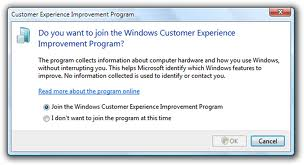
\includegraphics[scale=.5]{chapter8.tex/dialog6}
}
\caption{Dialog Box with Hyperlink}
\label{dialog6}
\end{figure}


Is it more confusing if I move the ``cancel'' button in  \autoref{dialog7}?  Will the user even see the ``cancel'' button? Will they become confused because the design conflicts with expectation?


\begin{figure}
\centerline{
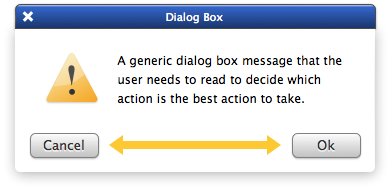
\includegraphics[scale=.5]{chapter8.tex/dialog7}
}
\caption{Button Layout}
\label{dialog7}
\end{figure}


Considering the examples above, it's easy to see how UI and software designers are able to easily break such a design pattern by:

\begin{itemize}
\item Packaging the information differently (adding more to a screen or component, for example)
\item Altering text on labels
\item Altering the position of a component so it is not in a familiar position
\item Creating a semantic mis-match between text and button labels
\end{itemize}

In a study of scalar implicature,  \citet*{Geurts:2009fw}  compared an inference task with a verification task and found that there was a positive response bias in the inference task not seen in the verification task. Under what situations might a modal dialog be better stated as a verification dialog than an  interrogative?\footnote{However, \citep{CliftonJr:2010dt} argue that the \citet{Geurts:2009fw} task (and corresponding interpretation of results) is flawed.}  One direct follow-up to Experiment 1 would be a follow-up to see if a verification dialog box reduces unwanted implicature.

Common design patterns are easily broken. Any designer or developer with a text editor can easily make changes without understanding the impact on comprehension. Producing comprehensible GUIs requires as much practice as writing clear, well-structured text. Design patterns arguably serve as a cognitive aid, boosting mechanisms supporting routinization and automatization of understanding. But as designers we need to be sensitive to the effect of alteration, no matter how benign the change might seem. We learn such sensitivity writing prose. It is time to take a hard look at micro-interactional design patterns and question what we think we know.

\subsection{Interactive Ads}
\label{interactiveads}

There is also ample room to continue exploration of deixis in graphical advertisements, as well. A next step would be to design follow-ups where advertisements are presented in isolation, in a manner similar to the pre-pilot for Experiment 2. Though Flash-based advertisements are becoming more rare, HTML5 is sufficiently richly interactive to expect ads will become increasingly interactive over time. And as we saw in Chapter 3, cross-media interactive advertising is already upon us.

How will such advertisements be perceived by users over time?  \citet{Goldstein:2013ww}  used AMT to study the cost of ``annoying ads'' on subjects. Prior research indicates, while there may be beneficial effects to small amounts of animation, too much may have a detrimental impact on ad effectiveness  \citep{Dreze:2003is,Goldfarb:2011kh,Buscher:2010uo}. \citet{Goldstein:2013ww}  studied the effect of annoying ads in an email sorting task. They believe that there may be a real cost beyond annoyance.

A key observation made in Experiment 2 was that embedded icons did not trigger inference of indexicality while in the context of an online news article. ``Pointing'' through animation might be effective for getting a user's attention, but this needs to be presented in such a way to avoid ``annoyance''. Regardless, micro-interactive graphics, including advertisements, are a rich new area for study. As hinted in Chapter 3, the rise of both behavioral advertising and interactive advertising in tandem will likely lead to new way to persuade and manipulate.

\subsection{Display Adaptation}
\label{displayadaptation}

Technology outpaces our ability to adapt standards for interaction. If the AdChoices icon was difficult to see and understand in a desktop browser, what does it look like in a mobile browser?


\begin{figure}
\centerline{
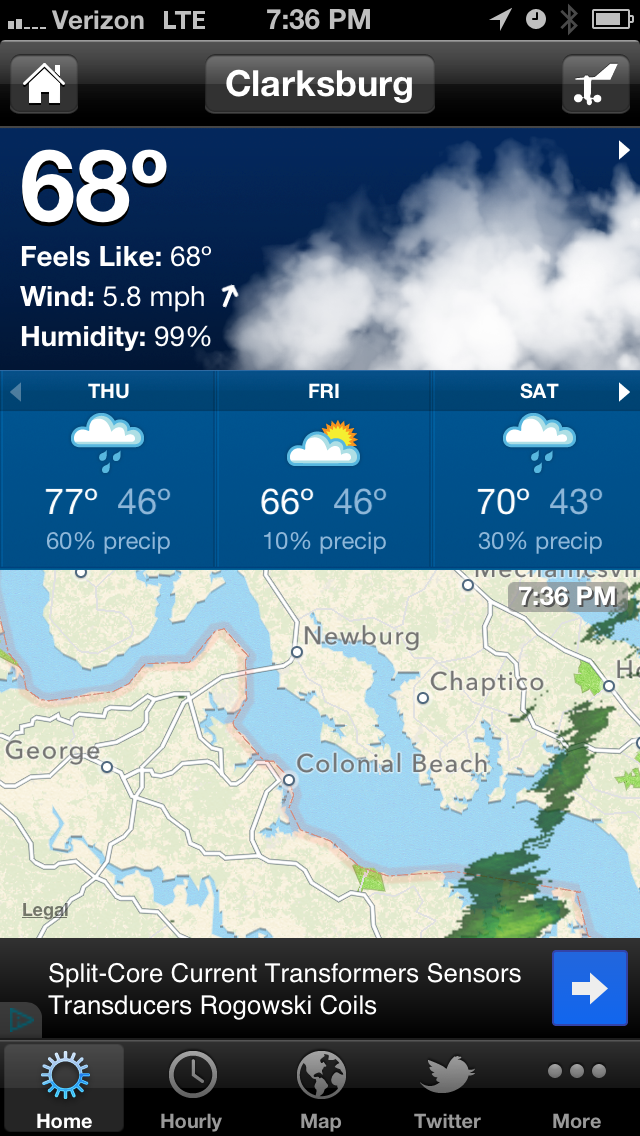
\includegraphics[scale=.2]{chapter8.tex/adchoices-mobile}
}
\caption{AdChoices Icon in iPhone Browser}
\label{adchoices}
\end{figure}


Try as I might --- I could not select the AdChoices icon in  \autoref{adchoices}  nor was there an obvious way to expand the advertisements size. 

What about the iconic buttons advertisers so like? Do they look out of place on the display in  \autoref{moble-button}? 


\begin{figure}
\centerline{
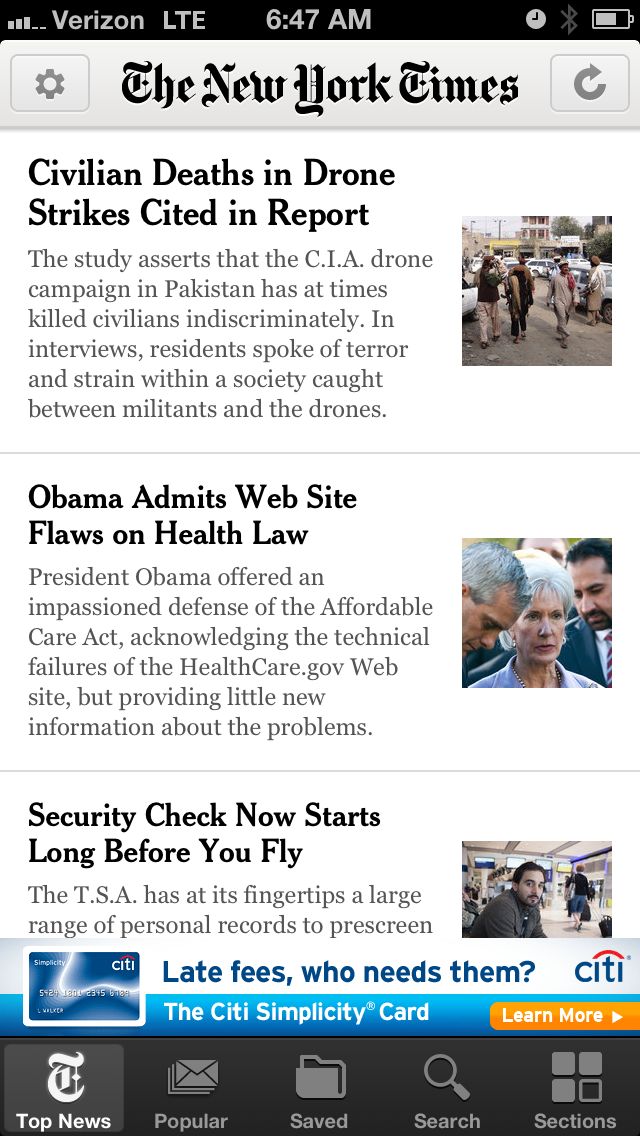
\includegraphics[scale=.2]{chapter8.tex/button-mobile}
}
\caption{Iconic Button in iPhone Browser}
\label{moble-button}
\end{figure}


Finally, its important to note that visual cues that we typically rely on for signaling an element on the page is interactive are beginning to disappear from touch-interactive displays.  \autoref{washpost}  is a page from the Washington Post application on the Apple iPad.


\begin{figure}
\centerline{
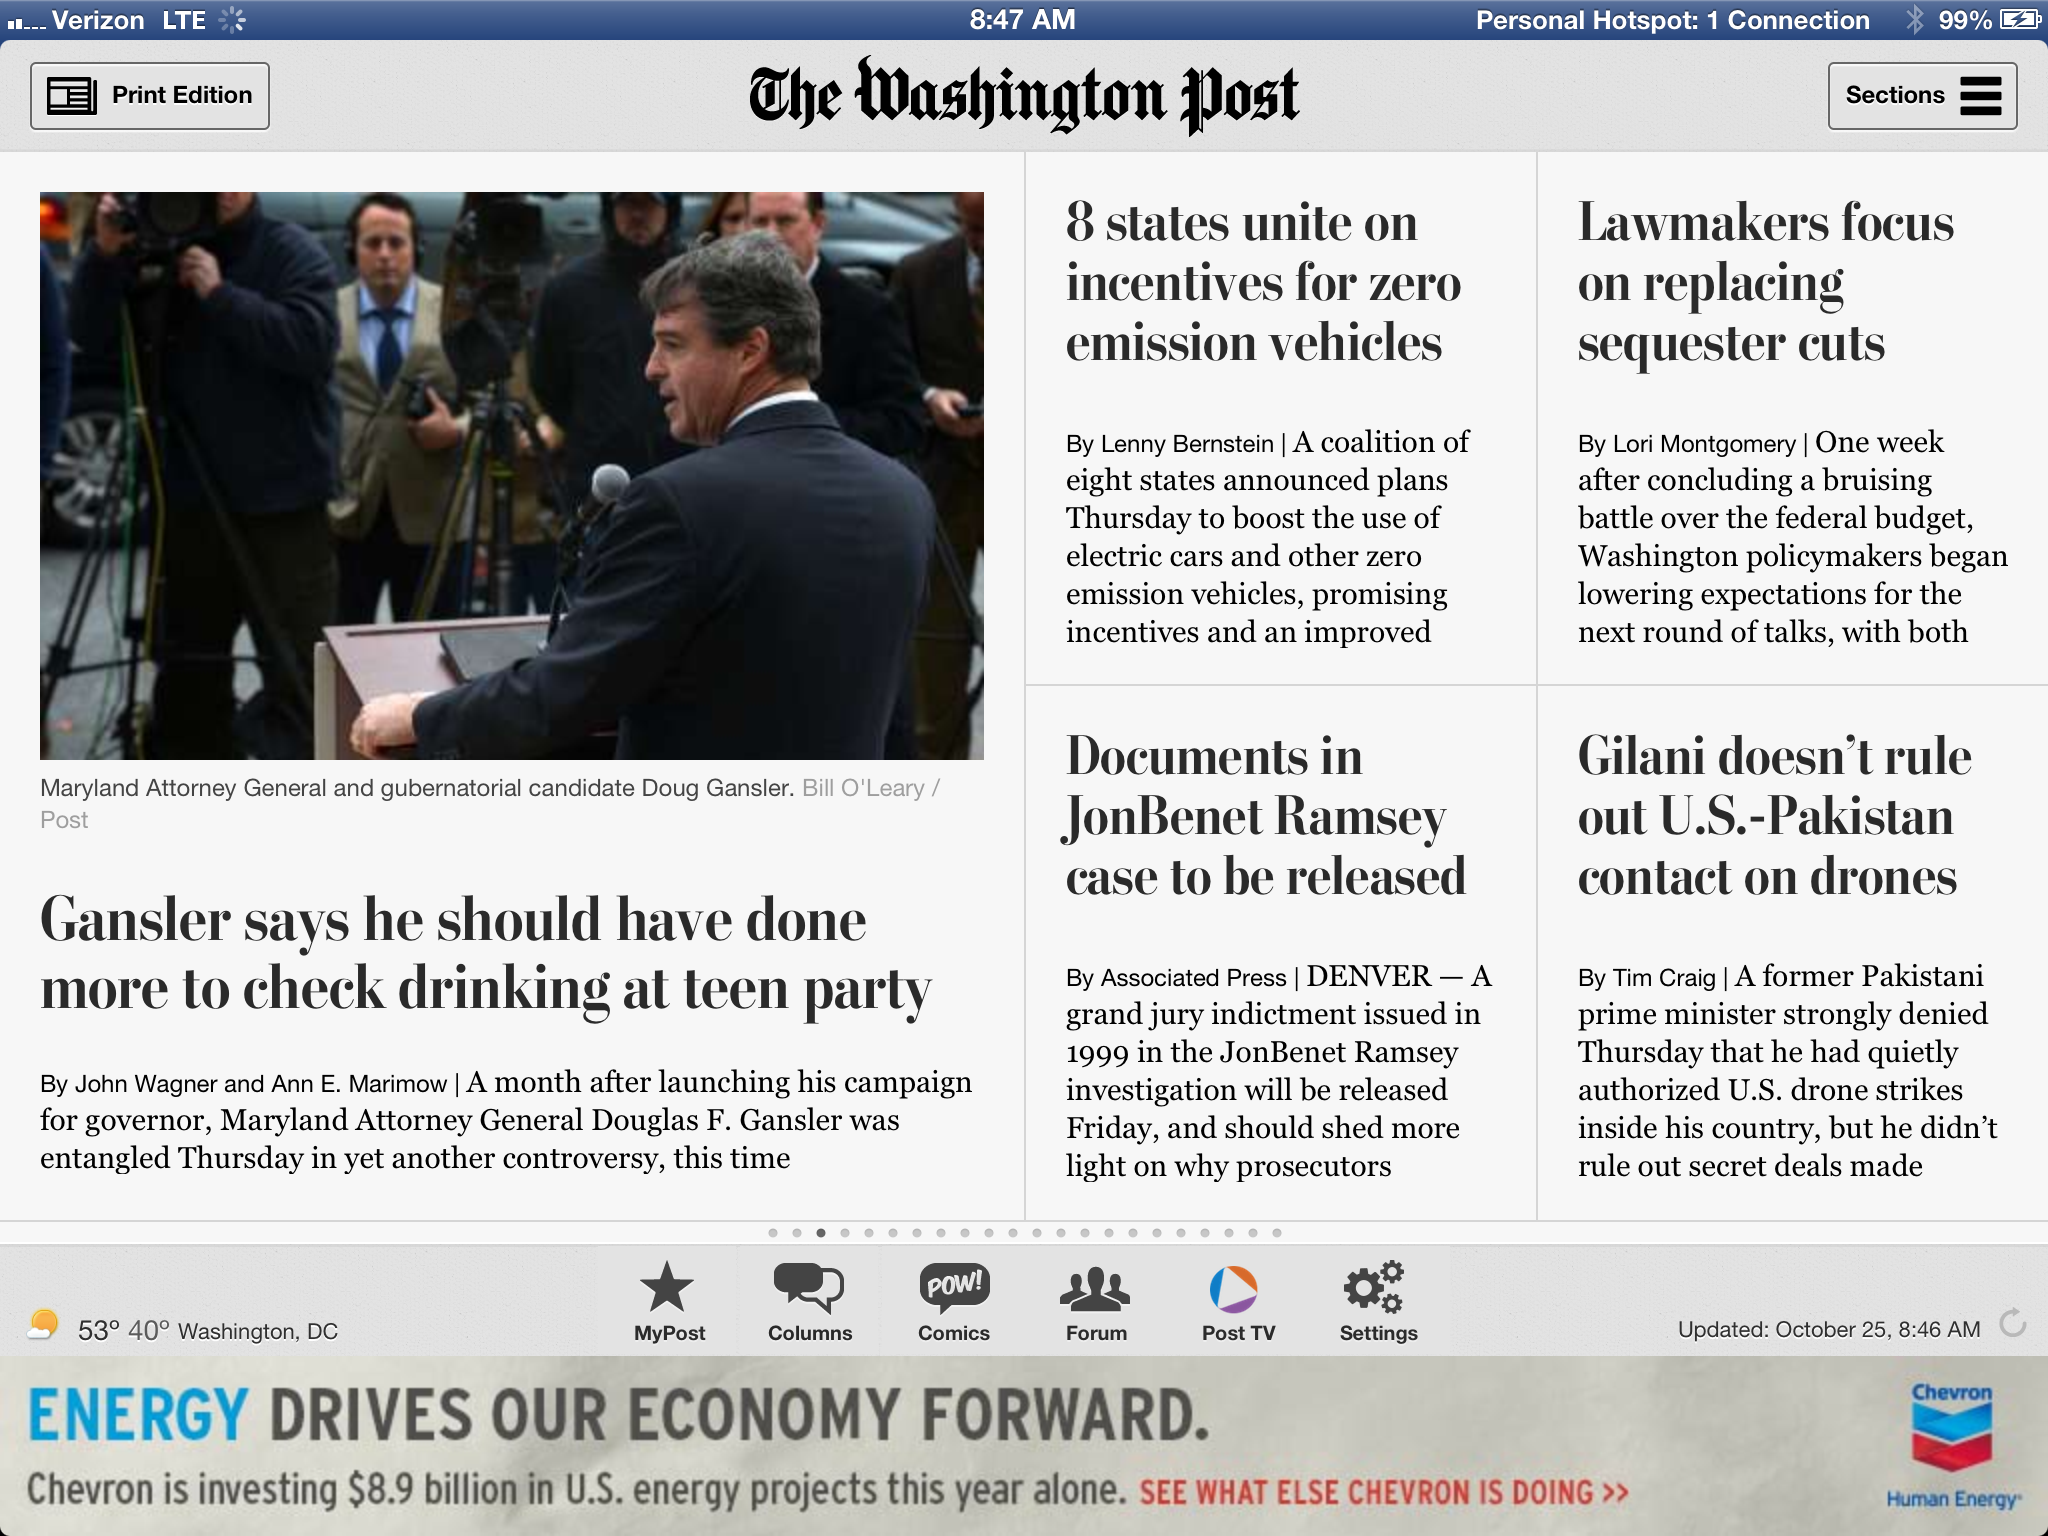
\includegraphics[scale=.1]{chapter8.tex/wash-post}
}
\caption{Washington Post on the iPad}
\label{washpost}
\end{figure}


Nowhere do you see blue text indicating textual hyperlinks. Once you dive into an article, such links are present. But presentation patterns in mobile devices are shifting expectations over time. 

\subsection{Social Microinteractions}
\label{socialmicrointeractions}

Experiment 3 suggests two avenues of future research. First, while it may not be possible to study the effects of eavesdropping in AMT, studying how people intentionally tailor messages for overhearers seems practicable. For example,  \citet{Egelman:2009ut}  found that users adapted their purchasing behavior to the presence of privacy indicators when purchasing privacy-sensitive items. 

What if consumers were given the choice to receive micro-payments in return for sharing information about what they purchased? What if, for example, a consumer, while in an Amazon shopping cart, had the ability to choose from three levels of micro-payment in return for sharing information about purchases. The smallest micropayment might be used to advertise only that he shopped for a ``drugstore item'' on Amazon. A second level might convey that he shopped for a ``hair product for men''. Finally, a third higher-priced level might convey brand such as ``Touch of Grey''. Would that consumer adjust levels on the basis of privacy-sensitivity and price?

This is an example of social sharing not yet seen on the Internet. Yet it is a plausible interaction. People are becoming more accustomed to tailoring messages to audiences on FaceBook, Google Plus and other social platforms. The challenge is that, while we may think this gives us finer-grained control over privacy, this may not be true.  \citet{Stutzman:2010ds}  found that while Facebook users have over time exhibited increasing privacy-seeking behavior (decreasing the amount of personal data shared publicly), the amount and scope of personal information they have revealed privately to other connected profiles has increased over time. And, as a result, so have disclosers to ``silent listeners'' --- third-party apps, and advertisers. While the impression is that users have greater and finer-grained control over privacy, the reality is that much of this is illusion. 

A second potential avenue for increasing social control over privacy is discussed below. Potentially, more transformative, is the need to redesign browser technology to reflect the nature of Internet browsing as inherently social --- that is, while it may be evident we are ``conversing'' with a particular website, third party participants may be unseen and present. Embracing a physical metaphor of spatial awareness may engender new styles of interaction for users seeking greater control over privacy.

\subsection{Socially Aware Browsers}
\label{sociallyawarebrowsers}

Technology has made it possible to engage in large-scale surveillance in the Internet and piece together little bits of behavioral data in the browser in order to create fairly accurate consumer profiles.\footnote{Most recently, it appears that political parties are using these techniques, and purchasing consumer data, in order to better target voters  \citep{Duhigg:2012uk}. } If one party (the publisher) has given consent for monitoring, U.S. law does not consider this as eavesdropping. Nonetheless, users find such monitoring ``creepy'' and invasive. When ads follow us across sites, it feels like eavesdropping. While browsing the Internet may feel anonymous and private, it is not. Despite lukewarm attempts by the advertising industry to self-regulate, the burden is on the user rather than the publishers and advertisers to opt-out of tracking. Furthermore, in the presence of a do not track signal from the user's browser, advertisers still intend to track, though they \emph{may not} display targeted advertising. Of course the potential harm is that any information collected this way may be wrong. Users have no way to know what is collected, what is right or wrong, or who may use this data and for what purpose.

A fundamental problem is this: despite bombardment by privacy policies that may mention ``affiliates'' and third-party trackers, while users are in the process of interacting online, they are not perceptually aware of such participants --- whether they are present are not. Overhearers are hidden inside of an HTTP request. Undoubtedly, the legal system will spend long years grappling with out-of-date privacy and data protection laws. In the meanwhile, we have an opportunity to change the current paradigm by making browsers more socially aware. That is, by acknowledging that interaction in a web browser is inherently multi-party, we can change the user experience to make transparent the social role of all participants present. The challenge is not to disrupt or annoy the user, but to keep such social awareness in the periphery. Social awareness should operate in real time and on a continuous basis. Perhaps, a good metaphor is a social network in the sense of Facebook or Google+. Showing the user who is present, who is a ``friend'', who ``friends'' of ``friends'' may be, and blocking un-ratified participants should be as natural as turning one's head to see who is close and lowering one's voice for better privacy. This does not solve the myriad of privacy problems associated with online behavioral tracking, but might at least afford users the chance to select an appropriate communication strategy for overhearers.
